\chapter{Marco Teórico} % Write in your own chapter title
\label{Chapter6}
\lhead{Capítulo 6. \emph{Marco Teórico}}

\section{Theoretical framework}

\subsection{State of the art}
\subsubsection{Automatic Plant diseases detection}

Plant disease classification is a very complex task as it relies on experts hands, but there are some automatic systems for the automatic detection of diseases, image processing, machine learning, and deep learning are some use-full tools to help in these tasks (see figure \ref{fig:detec}). Up to now most of the approaches for plant disease detection were depending on machine learning algorithms, these approaches are easily adapted to certain conditions as light for instance,  if the system has a new input with a tiny variation the accuracy of the model will decrease\cite{inbook}. The development of deep learning, deeper networks, convolutional neuronal networks (CNN) and transfer learning approach creates new models that are not as susceptible as common machine learning techniques.
\begin{figure}[h]
\centering
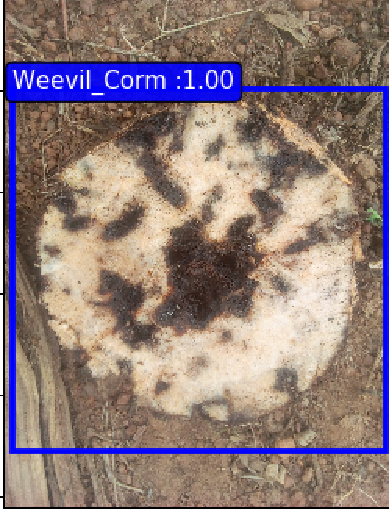
\includegraphics[scale=0.6]{Figures/result1.pdf}
\caption{Automatic pest detection in Banana using deep learning}
\label{fig:detec}
\end{figure}

\subsubsection{Pattern recognition}

Pattern recognition is a big knowledge area and is used in several applications in real life such as modelling, data management, commerce and even in politics. Disease diagnosis and detection are important topics to explore with pattern recognition and they have shown good results\cite{zhang2013nmr,felson1979new} also with techniques as machine learning\cite{kononenko2001machine,sajda2006machine}. Recently all these techniques are being applied in agriculture applications, starting with crop modeling \cite{bannayan2009using} , using support vector machines for crop classification \cite{camps2003support} and for plant disease detection \cite{rumpf2010early}.

\subsubsection{Deep learning}

Starting from machine learning networks, the necessity to create robust models, capable to manage several training classes, great inference power and good performance, made machine learning networks to grow in the sense of these new networks are deeper. For example in the ImageNet challenge(2012), AlexNet had a good performance\cite{NIPS2012_4824}. deep learning networks are working in important areas as face detection and agriculture, being this last a promising field to apply those techniques. Deep learning is used in Plant stress phenotyping\cite{SINGH2018883}, Plant diseases and pests detection in tomato\cite{article} ,Cassava disease detection\cite{ramcharan2017deep}\cite{sladojevic2016neural}, finally deep learning can be embedded into smartphones to create useful applications helping with disease diagnosis\cite{ramcharan}.

\subsubsection{Object detection} 

Classification in deep learning tasks aims to predict a class inside an image, for instance, if it is wanted to differentiate between if what there are in the images is a cat or a dog, the model can predict which animal it is. Object detection not just classify between a cat or a dog but detects where inside the image is the detected object (see figure \ref{fig:Spectral_Signature}), in this way, the system may tell the farmer where the disease is in a real scenario\cite{article}.Two examples of this technology in a real scenario are in Cassava and tomato, where object detection and transfer learning were used to detect diseases in the cassava and tomato leaves\cite{ramcharan}\cite{article} and implemented as a mobile application\cite{ramcharan2017using}. Currently, convolutional Neural Networks (CNN) are considered as the foremost method for object detection and there are some well performed methodologies such as Faster R-CNN and Single Shot Detectors (SSD). The evaluation of the performance is different from classification techniques as confusion matrix, there are some techniques to do the evaluation as mean average precision (mAP) score.

\begin{figure}[h]
\centering
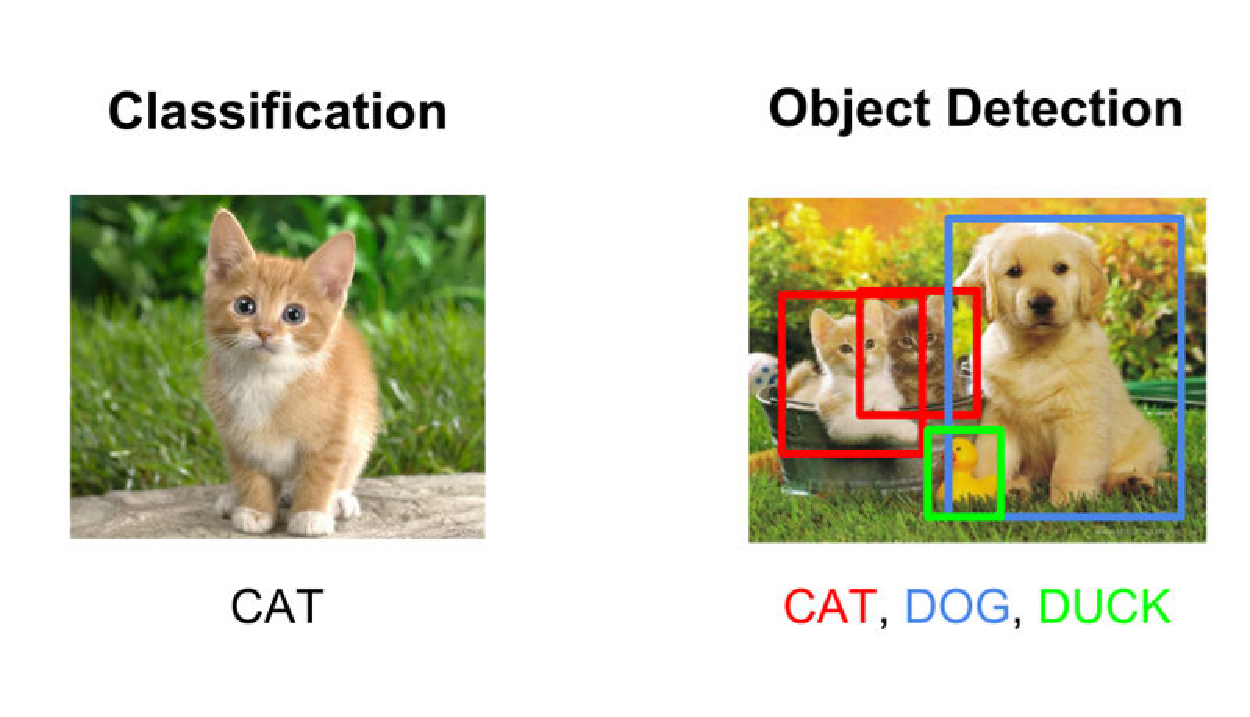
\includegraphics[scale=0.4]{Figures/object.pdf}
\caption{Difference between classification and object detection. From: Datacamp.[Online] Available at: https://www.datacamp.com/community/tutorials/object-detection-guide}
\label{fig:Spectral_Signature}
\end{figure}

\subsubsection{Transfer learning}

Transfer learning is becoming into an exciting way to face poor data situations \cite{pan2010survey}, is well known that for deep learning is needed huge data to train the network, what transfer learning is giving is a new technique to take pre-trained networks and adapt them to do a new task \cite{torrey2010transfer}. For instance, an existing network trained to classify cars can be re-trained to classify trucks without a training process from scratch, reducing the training time and getting faster results. 

\subsubsection{Generative adversarial networks}

GAN models are part of artificial intelligence, they are part of non supervising learning approaches which creates a system with two neuronal networks that compete with each other, were created by Ian Goodfellow et al. in 2014 \cite{NIPS2014_5423}. GAN models are currently being used in different applications: Style based generator architecture \cite{DBLP} that is a work from NVIDIA's team capable to generate artificial information based on two images and creating a new one with the mixing of features from both  images. Another  application is creating super resolution images\cite{DBLP1}. In conclusion, GAN models can generate artificial data to augment a data set to train deep learning models.

\subsubsection{Traditional data augmentation techniques}
Some machine and deep learning problems requires a data set with hundred or thousand of images, which is hard to collect in most of the cases, but with few images can be generate new samples to train the models applying different techniques\cite{barbedo2018impact} such as:
\begin{itemize} 
\item Vertical and horizontal flipping  
\item Image rotations
\item Brightness decrease and brightness increase
\item Contrast enhancement and contrast reduction
\item Sharpness enhancement
\item Addition of random Gaussian noise
\end{itemize}   

Those traditional techniques make models more robust and invariant to some variables as light condition and angle rotation, increasing the accuracy of the model.